\chapter{Implementacija i korisničko sučelje}
		
		
		\section{Korištene tehnologije i alati}
		
			 {Za komunikaciju unutar tima koristili smo \textbf{Whatsapp}\footnote{\url{https://www.whatsapp.com/}} i \textbf{Discord}\footnote{\url{https://discord.com/}}. Za izradu UML dijagrama koristili smo: \textbf{dbdiagram}\footnote{\url{https://dbdiagram.io/}} za dijagram baze podataka, \textbf{Visual Paradigm Online}\footnote{\url{https://online.visual-paradigm.com/}} za dijagram razreda te \textbf{Astah}\footnote{\url{https://astah.net/}} za ostale UML dijagrame. Kao sustav upravljanja verzijama je korišten \textbf{Git}\footnote{\url{https://git-scm.com/}} te su naši repozitoriji bili dostupni na \textbf{Githubu}\footnote{\url{https://github.com/}} udaljenom repozitoriju.
			 	
		 	Kao razvojno okruženje je korišten \textbf{PyCharm}\footnote{\url{https://www.jetbrains.com/pycharm/}} za razvoj API-ja te \textbf{Android Studio}\footnote{\url{https://developer.android.com/studio}} za razvoj mobilne aplikacije. Pycharm je razvojno okruženje za python, napravljeno od JetBrains-a te Android Studio je modificirana inačica drugog JetBrains razvojnog okruženja (IntelliJ, razvojno okruženje za Javu), prilagođena razvoju android mobilnih aplikacija.
		 	
		 	Mobilna aplikacija je napravljena s pomoću \textbf{Flutter}\footnote{\url{https://flutter.dev/}} razvojnog okvira koji koristi \textbf{Dart}\footnote{\url{https://dart.dev/}} programski jezik. Flutter i Dart su projekti razvijeni od strane Googlea. Flutter je razvojni okvir za izradu aplikacija na različitim platformama, vrlo popularan zbog mogućnosti kreiranja aplikacije za više platforma paralelno. Dart je moderni programski jezik koji se primarno koristi za razvoj Flutter aplikacija.
		 	API je kreiran s pomoću \textbf{Pythona}\footnote{\url{https://www.python.org/}} te \textbf{FastAPI}\footnote{\url{https://fastapi.tiangolo.com/}} razvojnog okvira. FastAPI je novije razvojno okruženje bazirano na Flasku, vrlo popularnom python razvojnom okruženju, s mogućnosti paralelnog izvođenja zahtjeva te automatskom dokumentacijom po OpenAPI standardu.
		 	
		 	Aplikacija je puštena u pogon na \textbf{Renderu}\footnote{\url{https://render.com/}}, te je korišten \textbf{Microsoft Azure}\footnote{\url{https://azure.microsoft.com/}}.
	 	 	za spremanje slika, za prepoznavanje teksta na slikama te se tamo nalazi naša baza podataka.
			 }
			 		
			\eject 
		
	
		\section{Ispitivanje programskog rješenja}
			
			\textbf{\textit{dio 2. revizije}}\\
			
			 \textit{U ovom poglavlju je potrebno opisati provedbu ispitivanja implementiranih funkcionalnosti na razini komponenti i na razini cijelog sustava s prikazom odabranih ispitnih slučajeva. Studenti trebaju ispitati temeljnu funkcionalnost i rubne uvjete.}
	
			
			\subsection{Ispitivanje komponenti}
			%\textit{Potrebno je provesti ispitivanje jedinica (engl. unit testing) nad razredima koji implementiraju temeljne funkcionalnosti. Razraditi \textbf{minimalno 6 ispitnih slučajeva} u kojima će se ispitati redovni slučajevi, rubni uvjeti te izazivanje pogreške (engl. exception throwing). Poželjno je stvoriti i ispitni slučaj koji koristi funkcionalnosti koje nisu implementirane. Potrebno je priložiti izvorni kôd svih ispitnih slučajeva te prikaz rezultata izvođenja ispita u razvojnom okruženju (prolaz/pad ispita). }
			
			{Ispitivanje funkcionalnosti sustava provedeno je uz pomoć unit testova. Testirani su service razredi te pripadajući routeri. U nastavku je priloženo nekoliko primjera tih testova te prikaz rezultata testiranja u razvojnom okruženju.\newline}
			
			{Test za razred UserService kojim se testira ispravno kreiranje novog korisnika. Servisu se šalje objekt tipa UserCreate te u slučaju da direktor još ne postoji očekujemo da će povratna vrijednost biti objekt User s podacima o novom korisniku.}
			
\begin{lstlisting}[style=pythonstyle]
	user_create = UserCreate(email="mail@mail.com",	first_name="Test", last_name="Test", username="test", password="test", roles=[RolesEnum.ADMIN],)
	user = User(id=1, email="test@email.com", first_name="Test", last_name="Test", username="test", roles=[],)
	
	def test_register_user():
		mock_user_crud = Mock()
		mock_user_crud.create_user.return_value = user.model_dump()
		mock_user_crud.get_users_by_role.return_value = None
		db = Mock()
		
		user_service = UserService(db)
		
		with patch("app.services.users.UserCRUD", 
					return_value=mock_user_crud):
			result = user_service.register_user(user_create)
		
		mock_user_crud.create_user.assert_called_once_with(user_create)
		mock_user_crud.get_users_by_role.assert_not_called()
		assert result == user.model_dump()
\end{lstlisting}
			
			{Sljedećim testom za documents router testira se reakcija pokušaja dohvaćanja povijesti skeniranih dokumenata za korisnika koji nije ulogiran te se očekuje 'NotAuthenticated' iznimka od servera.}
			
\begin{lstlisting}[style=pythonstyle]
	def test_get_me_not_authenticated():
		response = client.get("/documents/me")
		assert response.status_code == 401
		assert response.json() == {'app_exception': 'NotAuthenticated', 'context': {}}
\end{lstlisting}

			{Test za razred DocumentService koji testira kreiranje dokumenta. Servisu šaljemo sliku i korisničko ime te ako je dokument uspješno kreiran očekujemo da će nam servis vratiti kreirani novi objekt tipa Document sa svim podacima o dokumentu.}
			
\begin{lstlisting}[style=pythonstyle]
	@patch("app.services.documents.detect_document", return_value="R123456 text")
	def test_create_document(detect_document):
		mock_document_crud = Mock()
		mock_document_crud.create_document.return_value = document1
		
		mock_user_service = Mock()
		mock_user_service.get_user.return_value = admin
		
		mock_image_service = Mock()
		mock_image_service.create_image.return_value = imageDB
		db = Mock()
		
		document_service = DocumentService(db)
		
		with patch("app.services.documents.DocumentCRUD", return_value=mock_document_crud), patch("app.services.documents.ImageService", return_value=mock_image_service), patch("app.services.documents.UserService", return_value=mock_user_service):
			result = document_service.create_document(uploaded_image, "username")
		
		detect_document.assert_called_once()
		mock_user_service.get_user.assert_called_once()
		mock_image_service.create_image.assert_called_once()
		
		assert result == document1
\end{lstlisting}

			{Sljedeća dva testa testiraju ažuriranje statusa dokumenta u razredu DocumentService. Prvi provjerava dozvoljeni slučaj iz APPROVED želimo status postaviti na AUDITED, stoga nakon što servisu pošaljemo id dokumenta novi status te eventualne promjene u samom tekstualnom sadržaju očekujemo da će nam vratiti taj dokument s novim statusom. Drugi provjerava slučaj u kojem smo nakon statusa APPROVED odmah skočili na status ARCHIVED. Budući da to nije dozvoljeni slijed statusa očekujemo da će nam servis baciti iznimku "DocumentException.DocumentStatusNotCompatible".}
			
\begin{lstlisting}[style=pythonstyle]
	document2 = Document(id=2, image_id=1, owner=director, document_type=DocumentTypeEnum.INTERNAL, summary="test", document_status=DocumentStatusEnum.APPROVED, scan_time="2021-01-01T00:00:00",)
	document3 = Document(id=2, image_id=1, owner=director, document_type=DocumentTypeEnum.INTERNAL, summary="test", document_status=DocumentStatusEnum.AUDITED, scan_time="2021-01-01T00:00:00",)	

	def test_update_document():
		mock_document_crud = Mock(spec=DocumentCRUD)
		mock_document = Mock(spec=document2, document_status=DocumentStatusEnum.APPROVED)
		mock_document_crud.get_document.return_value = mock_document
		mock_document_crud.update_document.return_value = document3
		db = Mock()
		
		document_service = DocumentService(db)
		
		with patch("app.services.documents.DocumentCRUD", return_value=mock_document_crud):
		result = document_service.update_document(2, DocumentStatusEnum.AUDITED, None)
		
		mock_document_crud.update_document.assert_called_once()
		assert result == document3
	
	def test_update_document_with_invalid_status():
		mock_document_crud = Mock(spec=DocumentCRUD)
		mock_document = Mock(spec=document2, document_status=DocumentStatusEnum.APPROVED)
		mock_document_crud.get_document.return_value = mock_document
		mock_document_crud.update_document.return_value = document3
		db = Mock()
		
		document_service = DocumentService(db)
		
		with patch("app.services.documents.DocumentCRUD", return_value=mock_document_crud):
		with raises(DocumentException.DocumentStatusNotCompatible):
		document_service.update_document(2, DocumentStatusEnum.ARCHIVED, None)
\end{lstlisting}

			{Posljednji testovi testiraju arhiviranje dokumenta u sklopu ArchiveService-a. Dokument se smije arhivirati ako je prethodni status bio PENDING ili SIGNED\textunderscore PENDING. U prvom testu želimo arhivirati dokument čiji status arhiviranja je PENDING te ga želimo postaviti na DONE što je dozvoljeni slijed statusa. Očekuje se uspješni završetak metode archive\textunderscore document koja onda vraća arhivirani dokument s novim statusom DONE.
			U drugom testu želimo isprobati slučaj u kojem pokušavamo dokument iz AWAITING\textunderscore SIGNATURE statusa pretvoriti u DONE što nije dopušteni slijed stanja pa je i očekivano bacanje iznimke "ArchiveException.IllegalArchiveStatus".}
			
\begin{lstlisting}[style=pythonstyle]
	def test_archive_document():
		mock_archive_crud = Mock()
		mock_archive_crud.get_archived_by_document_id.return_value = archive1
		mock_archive_crud.update_archive.return_value = archive1
		
		mock_user_service = Mock(spec=UserService)
		mock_user_service.get_user.return_value = admin
		
		mock_document_service = Mock(spec=DocumentService)
		mock_document_service.update_document.return_value = None
		
		db = Mock()
		
		archive_service = ArchiveService(db)
		
		with patch("app.services.archives.ArchiveCRUD", return_value=mock_archive_crud):
			with patch("app.services.archives.UserService", return_value=mock_user_service):
				with patch("app.services.archives.DocumentService", return_value=mock_document_service):
					result = archive_service.archive_document(1, ArchiveStatus.DONE, "test")
		
		mock_archive_crud.get_archived_by_document_id.assert_called_once_with(1)
		mock_archive_crud.update_archive.assert_called_once()
		assert result == archive1
		
	def test_archive_document_forbidden():
		mock_archive_crud = Mock()
		mock_archive_crud.get_archived_by_document_id.return_value = archive3
		mock_archive_crud.update_archive.return_value = archive1
		
		mock_user_service = Mock(spec=UserService)
		mock_user_service.get_user.return_value = admin
		
		mock_document_service = Mock(spec=DocumentService)
		mock_document_service.update_document.return_value = None
		
		db = Mock()
		
		archive_service = ArchiveService(db)
		
		with patch("app.services.archives.ArchiveCRUD", 	return_value=mock_archive_crud):
			with patch("app.services.archives.UserService", return_value=mock_user_service):
				with patch("app.services.archives.DocumentService", return_value=mock_document_service):
					with raises(ArchiveException.IllegalArchiveStatus):
						archive_service.archive_document(1, ArchiveStatus.DONE, "test")
\end{lstlisting}

			{Svi navedeni ispitni slučajevi prošli su testiranje.}

			\begin{figure}[H]
				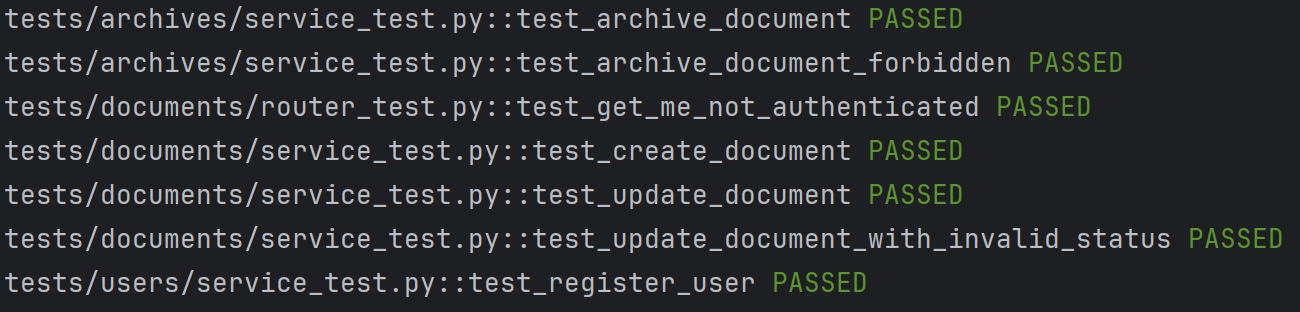
\includegraphics[width=\textwidth]{slike/unitTestovi.png}
				\caption{Prikaz rezultata ispitnih slučajeva u razvojnom okruženju}
				\label{fig:rezultatiUnitTestova}
			\end{figure}		
			
			
			\subsection{Ispitivanje sustava}
			
			 \textit{Potrebno je provesti i opisati ispitivanje sustava koristeći radni okvir Selenium\footnote{\url{https://www.seleniumhq.org/}}. Razraditi \textbf{minimalno 4 ispitna slučaja} u kojima će se ispitati redovni slučajevi, rubni uvjeti te poziv funkcionalnosti koja nije implementirana/izaziva pogrešku kako bi se vidjelo na koji način sustav reagira kada nešto nije u potpunosti ostvareno. Ispitni slučaj se treba sastojati od ulaza (npr. korisničko ime i lozinka), očekivanog izlaza ili rezultata, koraka ispitivanja i dobivenog izlaza ili rezultata.\\ }
			 
			 \textit{Izradu ispitnih slučajeva pomoću radnog okvira Selenium moguće je provesti pomoću jednog od sljedeća dva alata:}
			 \begin{itemize}
			 	\item \textit{dodatak za preglednik \textbf{Selenium IDE} - snimanje korisnikovih akcija radi automatskog ponavljanja ispita	}
			 	\item \textit{\textbf{Selenium WebDriver} - podrška za pisanje ispita u jezicima Java, C\#, PHP koristeći posebno programsko sučelje.}
			 \end{itemize}
		 	\textit{Detalji o korištenju alata Selenium bit će prikazani na posebnom predavanju tijekom semestra.}
			
			\eject 
		
		
		\section{Dijagram razmještaja}
			
			\textbf{\textit{dio 2. revizije}}
			
			 \textit{Potrebno je umetnuti \textbf{specifikacijski} dijagram razmještaja i opisati ga. Moguće je umjesto specifikacijskog dijagrama razmještaja umetnuti dijagram razmještaja instanci, pod uvjetom da taj dijagram bolje opisuje neki važniji dio sustava.}
			
			\eject 
		
		\section{Upute za puštanje u pogon}
		
			{U narednim potpoglavljima objašnjeno je kako pokrenuti sve dijelove aplikacije lokalno ili postavljanjem na besplatne servise.}
		
			\subsection{Puštanje poslužitelja u pogon}
			\subsection{Puštanje mobilne aplikacije u pogon}
			
			{U naredna dva potpoglavlja dane su opcije pokretanja i izgradnje Flutter mobilne aplikacije te mogućnost objave.}
			
			\subsubsection{Instalacija potrebnih alata za pokretanje i lokalna izgradnja}
			
			{U nastavku je dan niz naredbi za lokalno preuzimanje i pokretanje aplikacije.}
			\begin{enumerate}
			\item{Namjestiti Flutter razvojni okvir i razvojno okruženje po želji koristeći službene upute\footnote{\url{https://docs.flutter.dev/get-started/editor}}}
			\item{Klonirati repozitorij s izvornim kodom lokalno pomoću Git naredbi}
			\item{Unutar src direktorija pokrenuti sljedeće naredbe}
			\begin{verbatim}
flutter pub get
flutter build apk --dart-define=APP_NAME=Digitalizacija 
--dart-define=BASE_URL=jura-hostic-i-film-api.onrender.com --release
			\end{verbatim}
			\end{enumerate}
			
			\subsubsection{Objava aplikacije na F-Droid platformi}
			
			{F-Droid je platforma za objavljivanje besplatnih mobilnih aplikacija s javno dostupnim izvornim kodom. Omogućava postavljanje vlastitih aplikacija predajom podataka za izgradnju iz javnog Git repozitorija i dijeljenja s pomoću metapodataka.}
			
			{U nastavku je dan niz uputa koje valja slijediti ako se aplikacija želi objaviti putem F-Droid platforme.}
			\begin{enumerate}
				\item{Izraditi GitLab\footnote{\url{https://about.gitlab.com/}} račun}
				\item{Izvršiti git fork nad fdroiddata\footnote{\url{https://gitlab.com/fdroid/fdroiddata}} repozitorijem}
				\item{Daljnje korake izvršiti u sklopu Linux okvira, za Windows operacijski sustav preporuča se upotreba WSL 2\footnote{\url{https://learn.microsoft.com/en-us/windows/wsl/install}} alata}
				\item{Preuzeti stvoreni repozitorij}
				\begin{verbatim}
git clone --depth=1 https://gitlab.com/IME_RACUNA/fdroiddata ~/fdroiddata
cd ~/fdroiddata
git checkout -b com.example
cp templates/build-flutter.yml metadata/com.example.jura_hostic_i_film_app.yml
				\end{verbatim}
				\item{Urediti com.example.jura\_hostic\_i\_film\_app.yml metadata datoteku po želji, preporuča se sljedeća konfiguracija}
				\begin{figure}[H]
					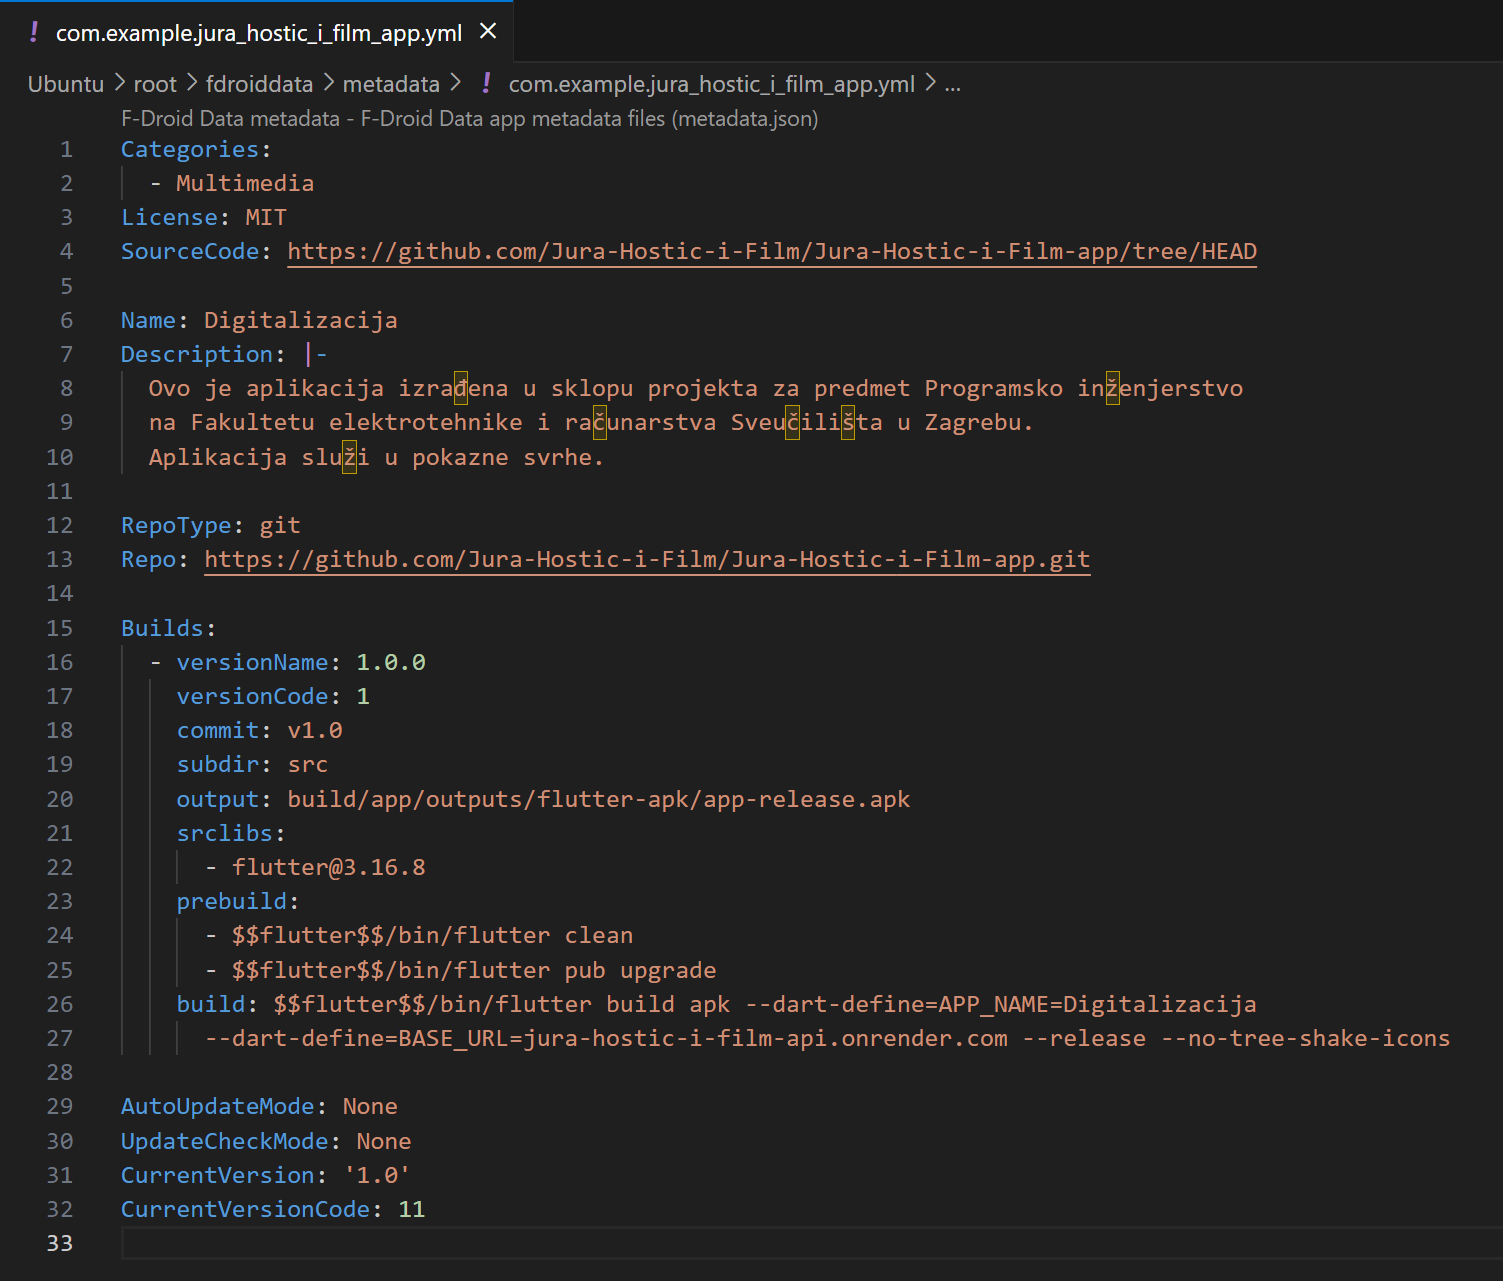
\includegraphics[width=\textwidth]{slike/metadata.png}
					\caption{Prikaz postavki u metadata datoteci}
					\label{fig:metadataPostavke}
				\end{figure}
				\item{Preuzeti zadnju inačicu kontejnera sa serverskim alatima, na Windows operacijskom sustavu dodatno treba instalirati Docker\footnote{\url{https://docs.docker.com/desktop/install/windows-install/}} alat i omogućiti uporabu unutar WSL 2 okruženja}
				\begin{verbatim}
git clone --depth=1 https://gitlab.com/fdroid/fdroidserver \
~/fdroidserver
sudo sh -c 'apt-get update &&apt-get install -y docker.io'
sudo docker run --rm -itu root --entrypoint /bin/bash \
-v ~/fdroiddata:/build:z \
-v ~/fdroidserver:/home/vagrant/fdroidserver:Z \
registry.gitlab.com/fdroid/fdroidserver:buildserver
				\end{verbatim}
				\item{Unutar kontejnera pokrenuti sljedeći niz naredbi}
				\begin{verbatim}
				. /etc/profile
export PATH="$fdroidserver:$PATH" PYTHONPATH="$fdroidserver"
export JAVA_HOME=$(java -XshowSettings:properties -version 2>&1 > \
/dev/null | grep 'java.home' | awk -F'=' '{print $2}' | tr -d ' ')
cd /build
fdroid readmeta
fdroid rewritemeta com.example.jura_hostic_i_film_app
fdroid checkupdates --allow-dirty com.example.jura_hostic_i_film_app
fdroid lint com.example.jura_hostic_i_film_app
fdroid build com.example.jura_hostic_i_film_app
				\end{verbatim}
				\item{Nakon uspješne izgradnje paketa izvršiti sljedeći niz naredbi}
				\begin{verbatim}
exit
cd ~/fdroiddata
git add metadata/com.example.jura_hostic_i_film_app.yml
git commit -m "New App: com.example.jura_hostic_i_film_app"
git push origin com.example
				\end{verbatim}
				\item{Na kraju otvoriti zahtjev za spajanje vlastite grane na fdroiddata repozitorij}
				\item{F-Droid tim može imati dodatnih pitanja u slučaju krivo provedenog postupa, stoga je bitno ostati na raspolaganju}
			\end{enumerate}
			
			{Prilikom izrade zahtjeva za objavu važno je pratiti konvencije kojih se pridržava F-Droid platforma, koje se zajedno sa svim dodatnim informacijama mogu naći na stranicama platforme. \footnote{\url{https://f-droid.org/docs/Submitting\_to\_F-Droid\_Quick\_Start\_Guide/}}}
			
			{U slučaju ispravne predaje zahtjev za objavu se obrađuje, F-Droid tim vrši verifikaciju te se aplikacija objavljuje u najkraćem mogućem vremenu.}
			
			\eject 